\documentclass{article}
\usepackage[UTF8]{ctex}
% Replace `letterpaper' with`a4paper' for UK/EU standard size
\usepackage[a4paper,top=2cm,bottom=2cm,left=3cm,right=3cm,marginparwidth=1.75cm]{geometry}

% Useful packages
\usepackage{amsmath}
\usepackage{mathrsfs,amsmath}
\usepackage{graphicx}
\usepackage[colorlinks=true, allcolors=blue]{hyperref}
\usepackage{graphicx} %插入图片的宏包
\usepackage{float} %设置图片浮动位置的宏包
\usepackage{subfigure} %插入多图时用子图显示的宏包
\usepackage{parskip}
\usepackage{indentfirst} 
\setlength{\parindent}{2em}
\usepackage{hyperref}  
\usepackage{tikz}
\allowdisplaybreaks
\usepackage{multirow}
\usepackage{amsmath}
\usepackage{amsfonts,amssymb} 
\usepackage{xcolor} % 用于显示颜色
\usepackage{listings} % 用于插入代码
\lstset{
	basicstyle          =   \sffamily,          % 基本代码风格
	keywordstyle        =   \bfseries,          % 关键字风格
	commentstyle        =   \rmfamily\itshape,  % 注释的风格,斜体
	stringstyle         =   \ttfamily,  % 字符串风格
	flexiblecolumns,                % 别问为什么,加上这个
	numbers             =   left,   % 行号的位置在左边
	showspaces          =   false,  % 是否显示空格,显示了有点乱,所以不现实了
	numberstyle         =   \zihao{-5}\ttfamily,    % 行号的样式,小五号,tt等宽字体
	showstringspaces    =   false,
	captionpos          =   t,      % 这段代码的名字所呈现的位置,t指的是top上面
	frame               =   lrtb,   % 显示边框
}

\lstdefinestyle{Python}{
	language        =   Python, % 语言选Python
	basicstyle      =   \zihao{-5}\ttfamily,
	numberstyle     =   \zihao{-5}\ttfamily,
	keywordstyle    =   \color{blue},
	keywordstyle    =   [2] \color{teal},
	stringstyle     =   \color{magenta},
	commentstyle    =   \color{red}\ttfamily,
	breaklines      =   true,   % 自动换行,建议不要写太长的行
	columns         =   fixed,  % 如果不加这一句,字间距就不固定,很丑,必须加
	basewidth       =   0.5em,
}

\title{图像处理与可视化 Homework-6 报告}
\author{林子开 21307110161}
\begin{document}
	\maketitle
	\tableofcontents

\section{图像分割:基于Kmeans算法}
\subsection{Python代码}
\lstinputlisting[style = Python,
caption={Python codes}]{exercise-1.py} 
\subsection{二分类,并与OTSU算法比较}
用于测试的图片(带$1\%$的椒盐噪声)如下:
\begin{figure}[H]
	\centering
	{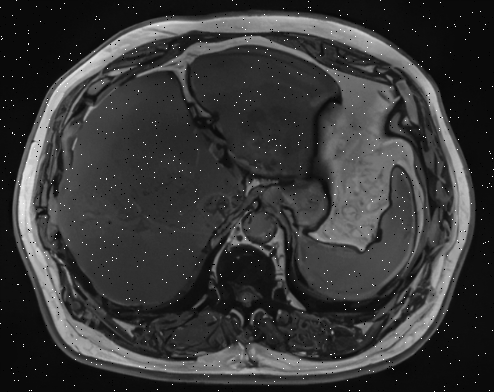
\includegraphics[width=0.5\textwidth]{受到椒盐噪声污染的肝脏图像.png}} 
	\caption{测试图像(带$1\%$的椒盐噪声)}
\end{figure}
用Kmeans做二类分割的效果如图\ref{k2}所示,用OSTU进行二值化的效果如图\ref{ostu}所示。
(注意,虽然用OSTU进行二值化的最终效果应该是黑白图片,但是为了与Kmeans统一,我将二值化后的结果为0的像素点
设置为橙色,将二值化后结果为255的像素点设置为蓝色,以便读者与kmeans进行比较。)
\begin{figure}[H]
    \centering
    \subfigure[Kmeans二类分割]
    {\label{k2} 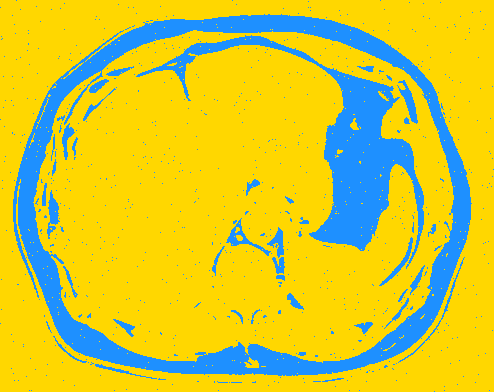
\includegraphics[width=0.47\textwidth]{exercise1_result//k=2.png}}
    \,    
    \subfigure[OSTU二值化]
    {\label{ostu} 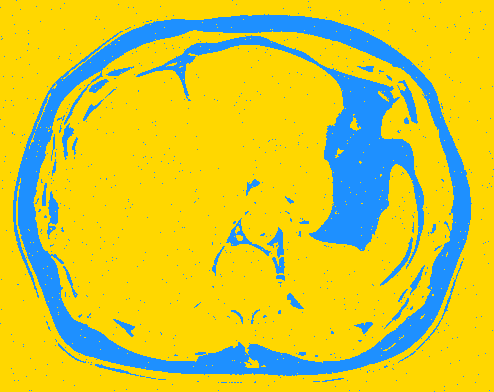
\includegraphics[width=0.47\textwidth]{exercise1_result//OTSU.png}}
    \caption{Kmeans和OSTU二值化效果对比}\label{} 
\end{figure}
可以看出,两个算法进行二类分割的\textbf{效果基本一致}。

\subsection{多分类}
多分类分割的效果如下所示
\begin{figure}[H]
    \centering
    \subfigure[k = 3]
    {\label{} 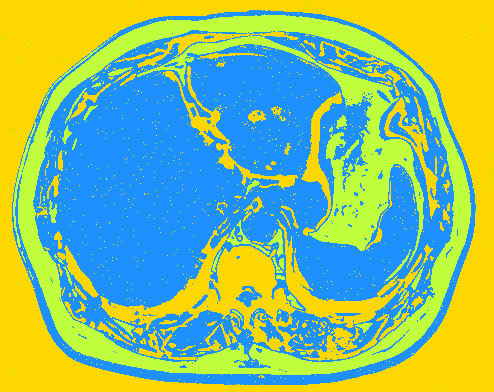
\includegraphics[width=0.45\textwidth]{exercise1_result//k=3.png}}
    \,    
    \subfigure[k = 4]
    {\label{} 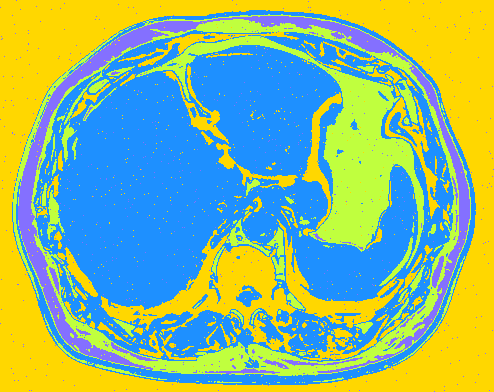
\includegraphics[width=0.45\textwidth]{exercise1_result//k=4.png}}
    \,
    \subfigure[k = 5]
    {\label{} 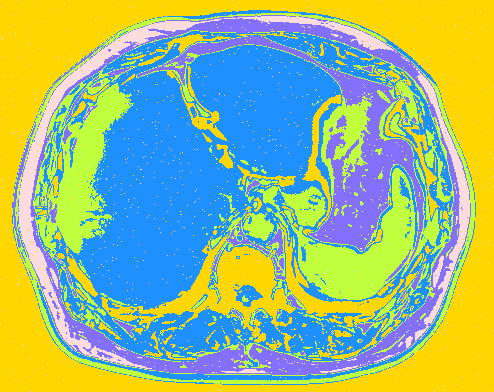
\includegraphics[width=0.45\textwidth]{exercise1_result//k=5.png}}
    \,    
    \subfigure[k = 6]
    {\label{} 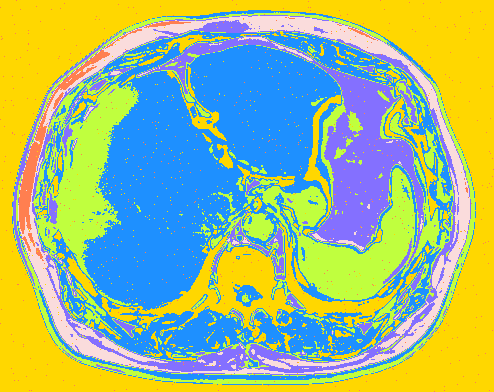
\includegraphics[width=0.45\textwidth]{exercise1_result//k=6.png}}
    \caption{多类分割效果}\label{} 
\end{figure}
可以发现,当$k=3$时,分类效果比较好。当$k>3$时,会分割出一些无意义的颜色类别。
\subsection{分析带噪声图像分类不准确的原因并提出改进措施}
椒盐噪声只分布在0和255两个灰度值上,因此在kmeans聚类时,带有椒盐噪声的像素点一定会被分到均值最低的类
或均值最高的类,因此带椒盐噪声像素点的分类是确定的。
另一方面,kmeans算法\textbf{并不考虑图像的空间信息},只是根据灰度值的大小对所有像素的灰度值进行聚类。
当某个像素点出现了椒盐噪声,算法并没有考虑到其周围像素点的信息,不管噪声所在像素点邻域内的
像素被分到了哪一类,都不会改变该噪声像素点的分类结果。
所以,在分割的图像中,我们会明显地看到噪声所在的位置被分配到了和其邻域像素点完全不同的类别中,
kmeans对带噪声的图像进行分割的能力并不好。

如果想要得到更好的分割结果,可以\textbf{先用中值滤波器对椒盐噪声先进行去噪操作,再进行分割}。
而对于其他类型的噪声,则要选取其他适合的滤波器,如高斯滤波器等,同样先去噪、后分割。

\newpage
\section{基于形态学操作进行补洞与噪声去除}
\subsection{Python代码}
\lstinputlisting[style = Python,
caption={Python codes}]{exercise-2.py} 
\subsection{操作结果}

先对图像用大小为$7\times 7$的正方形结构元进行闭操作,对孔洞进行填充;
再对图像用大小为$5 \times 5$的正方形结构元进行开操作,去除椒盐噪声。
效果如下:

% \begin{figure}[H]
% 	\centering
% 	{\includegraphics[width=0.99\textwidth]{zmic_fdu_noise.bmp}} 
% 	\caption{原图} 
% \end{figure}

\begin{figure}[H]
	\centering
	{
\includegraphics[width=0.99\textwidth]{exercise2_result//result.png}} 
	\caption{进行形态学处理后的图像}
\end{figure}


\end{document}

% \begin{figure}[H]
% 	\centering
% 	{\includegraphics[width=0.35\textwidth]{image//ignorance.png}} 
% 	\caption{} \label{} 
% \end{figure}


% \lstinputlisting[style = Python,
% caption={Python codes},
% label = {efficient},
% linerange={110-125}]{exercise3.py} 


% \begin{figure}[H]
%     \centering
%     \subfigure[patch size = 11]
%     {\label{} 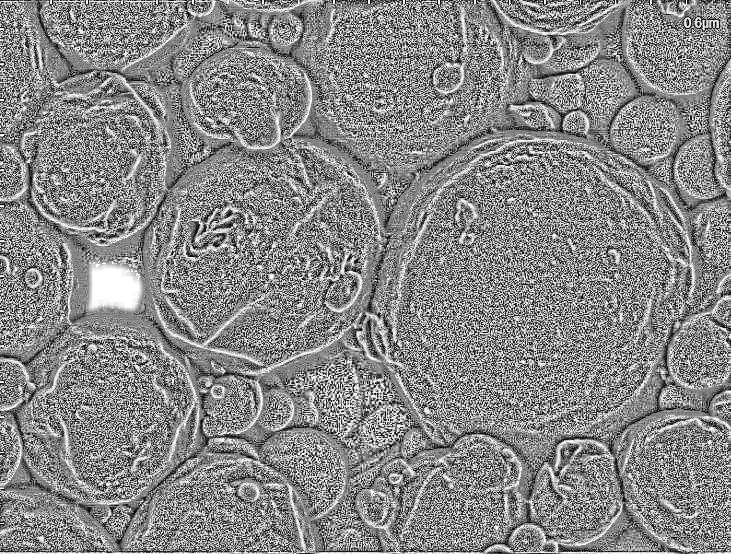
\includegraphics[width=0.49\textwidth]{image//local equalization with patch size = 11.jpg}}
%     \,    
%     \subfigure[patch size = 51]
%     {\label{} 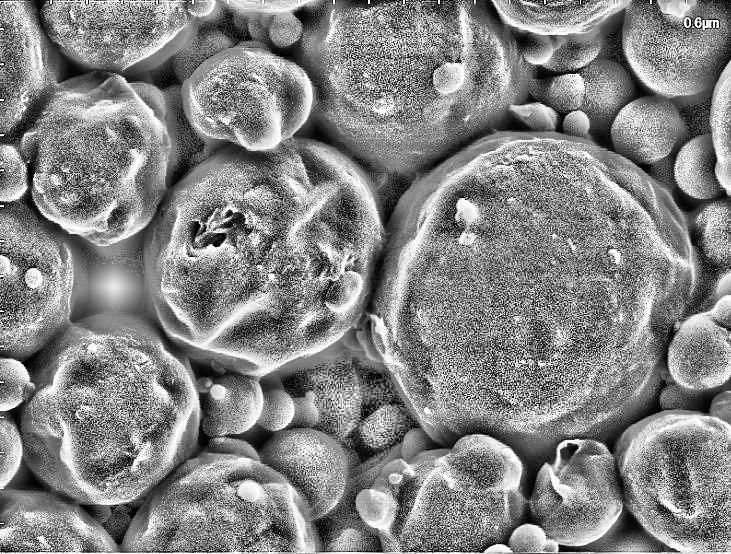
\includegraphics[width=0.49\textwidth]{image//local equalization with patch size = 51.jpg}}
%     \,
%     \subfigure[patch size = 151]
%     {\label{} 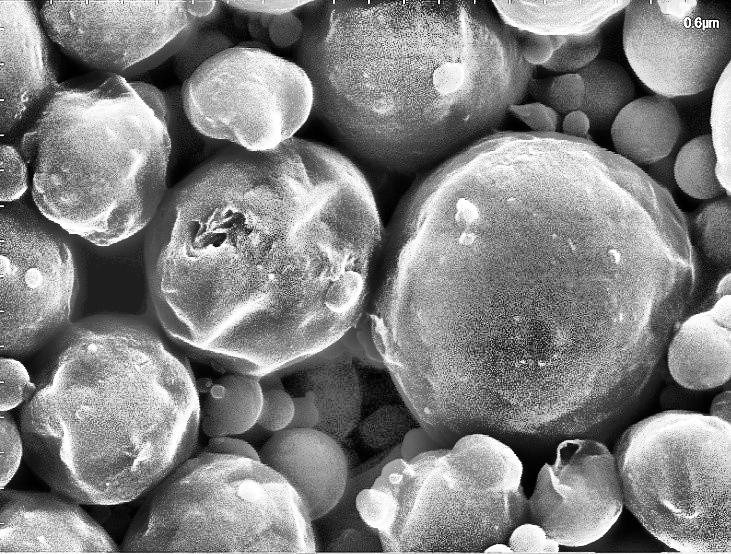
\includegraphics[width=0.49\textwidth]{image//local equalization with patch size = 151.jpg}}
%     \,    
%     \subfigure[patch size = 201]
%     {\label{} 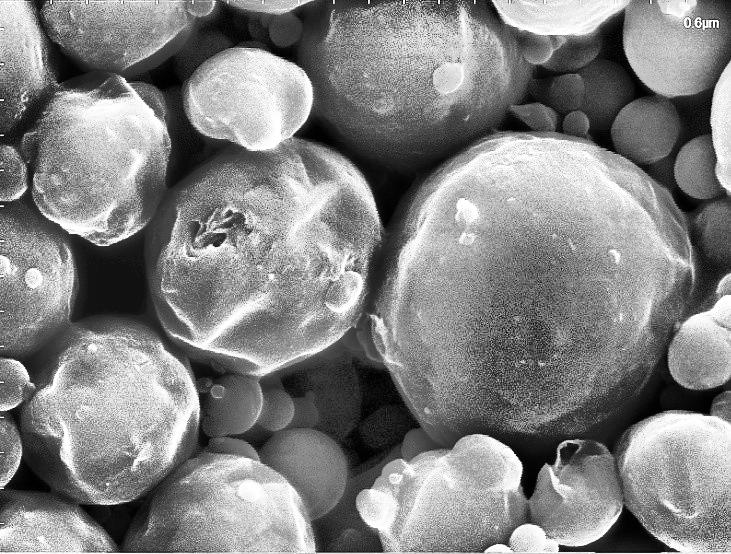
\includegraphics[width=0.49\textwidth]{image//local equalization with patch size = 201.jpg}}
%     \caption{local equalization with different patch sizes}\label{} 
% \end{figure}
